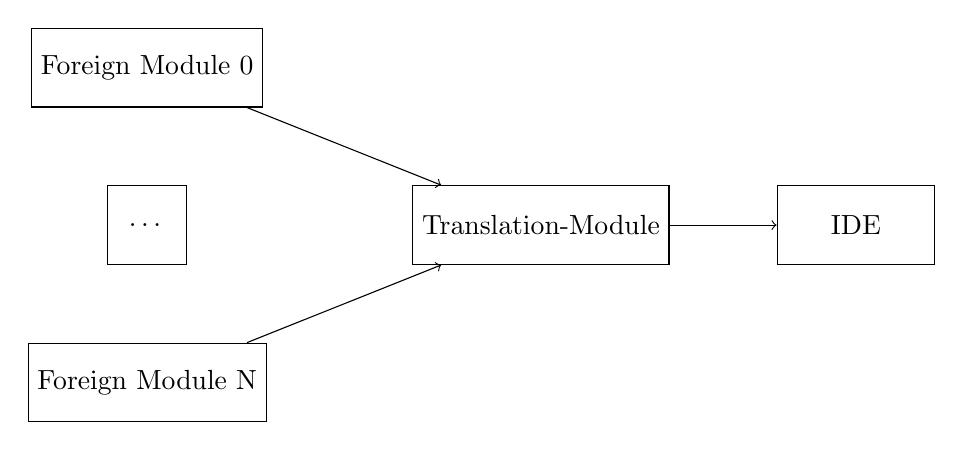
\begin{tikzpicture}
  % Nodes
  \node (p-0) [rectangle, draw, minimum height=1cm, minimum width=2cm] at (-6, 2) {Foreign Module 0};
  \node (dots) [rectangle, draw, minimum height=1cm, minimum width=1cm] at (-6, 0) {\dots};
  \node (p-n) [rectangle, draw, minimum height=1cm, minimum width=2cm] at (-6, -2) {Foreign Module N};
  \node (m) [rectangle, draw, minimum height=1cm, minimum width=2cm] at (-1, 0) {Translation-Module};
  \node (i) [rectangle, draw, minimum height=1cm, minimum width=2cm] at (3, 0) {IDE};
  % Arrow
  \draw[->] (m) -- (i);
  \draw[->] (p-0) -- (m);
  \draw[->] (p-n) -- (m);
  % Header
\end{tikzpicture}
